
%
% Use the standard article template.
%
\documentclass{article}

% The geometry package allows for easy page formatting.
\usepackage{geometry}
\geometry{letterpaper}

% Load up special logo commands.
\usepackage{doc}

% Package for formatting URLs.
\usepackage{url}

% Packages and definitions for graphics files.
\usepackage{graphicx}
\usepackage{epstopdf}
\DeclareGraphicsRule{.tif}{png}{.png}{`convert #1 `dirname #1`/`basename #1 .tif`.png}

%
% Set the title, author, and date.
%
\title{CMSI 370: The Longevity of the Hewlett-Packard 12c Calculator}
\author{Chris Whiting}
\date{}

%
% The document proper.
%
\begin{document}

% Add the title section.
\maketitle

% Add an abstract.
\abstract{
The success and popularity of a user interface can be attributed to its correct alignment of the user and developer mental models. The developer mental model is the designer's conceptual model. The user model is the mental model created from the user's interaction with the system. The system image is the physical result of the developer's mental model. The developer expects the user's mental model to be the same as the designer's mental model. When a user interacts with a system, they communicate with the system image.  However, if the system image does not accurately reflect the developer's mental model, then the user will end up with the wrong mental model for the system. The correct balance of the user's mental model, the developers mental model, and the system image is present in the Hewlett-Packard 12c Calculator. 
}

% Add various lists on new pages.
\pagebreak
\tableofcontents

% Start the paper on a new page.
\pagebreak

%
% Body text.
%
\section{Introduction}
\label{introduction}

The popularity and longevity of the HP 12c calculator can be attributed to the following factors: , specific functions for financial applications, the calculator's Reverse Polish Notation (RPN) style of data entry, and the ability to write programs. When using the hp12c, the user's mental model changes according to the specific operation being performed. When a calculation involving a specific financial function is being performed, the user's mental model consists of the givens, the unknowns, and the method of solving. The method of RPN is fun to use, and significantly decreases the amount of key presses by the user. Writing programs to fit any financial problem, lets the user create their own developer model, which therefore must equal the user's mental model. This is the most important factor of the hp12c, because it allows the user to create their own developer model and system image.


\section{Basic Financial Functions}

The basic financial functions of the hp 12c helps to simplify, ordinarily complex financial calculations. To accomplish this, the calculator utilizes special financial registers in memory. The memory of the hp12c also helps improve calculation efficiency along with the financial functions. The financial registers are designated by n, i , PV, PMT, and FV as shown in Figure Figure~\ref{financial-buttons}.

The n financial register denotes the number of days, i represents the annual interest rate, PV denotes the principal amount or present value, PMT is the register standing for the period payment, and the FV register represents the future value during calculations. Solving simple financial calculations is only a matter of keying the correct quantities in the cooresponding financial registers with the register buttons shown in Figure~\ref{financial-buttons}.

These registers represent the system image that is based on the developer's model. When the user attempts to solve a financial problem, they create a mental model based on the specific calculation required. The financial functions registers create a clearer system image from the developer's mental model, by allowing the user to systematically enter their calculation. 

Each step in solving a financial calcualtion will be envisioned by the user and thus the user's mental model is developed. The system image for the operation of the financial functions and registers align with the user's mental model, in terms of steps to reach the answer. That is, the steps the user envisions for any financial calculation can almost directly be keyed on the hp 12c with the financial functions and registers.

\begin{figure}
\centering
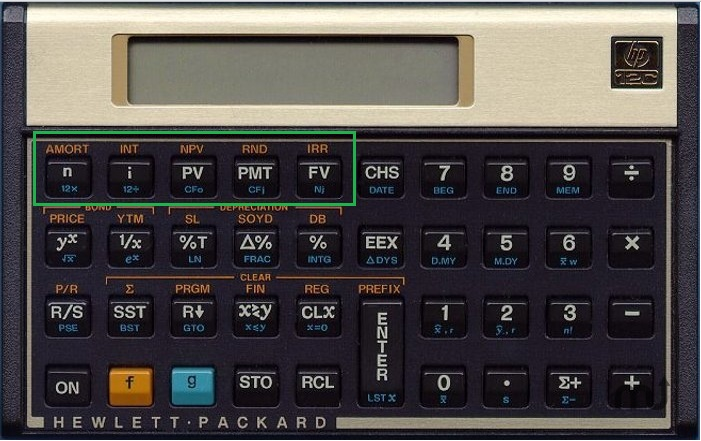
\includegraphics[width=3in]{Figure_1.jpg}
\caption{HP12c Financial Function Buttons}
\label{financial-buttons}
\end{figure}

\section{Reverse Polish Notation (RPN)}

A very efficient method of data entry that is used for the hp 12c calculator is Reverse Polish Notation. This style of data entry eleiminates the need to enter paratheses in equations by placing the operators before or after the operands. When a user thinks of a simple calculation to be performed through a calculator, the majority of users would think of the following input method:
\begin{verbatim}
   560
+  400
---------
   960
\end{verbatim}
The Reverse Polish Notation allows the user to enter the above math formula exactly how the user would think of it. That is, by pressing "560" ,"Enter",  "400" , and "+"  yields the result. The Enter key is used between operations when the user is finished keying in the first number. Multiple numbers may be added, subtract, multiplied, etc. in the same way shown above, where the operation is specified after the 2nd digit (postfix), instead if before the 2nd digit (prefix). The math expression above is evaluated exactly the same way as a user would think of solving the expression.

The developer's mental model for data entry on the hp 12c led to the system image of RPN. The user does not intereact with the developer's mental model, but in fact interacts with the system image, which is the RPN style of data entry. Therefore, because RPN allows the user to evauate an expression almost exactly the same way as their mental model suggests, the developer's mental model and the user's mental model successfully align.

\section{Writing Custom Programs}

Writing programs onto calculators is not new in today's world, however, the hp12c has the ability to write programs and also utilizes RPN data entry to more efficiently create lengthy programs. Programs are created and executed while the calculator is operating in Program mode, which displays a PGRM indicator on the screen, shown in Figure 2. Whenever the user starts to key in a program, each key is stored in program memory. 

When a program is executed the hp12c goes through each line of program memory and performs the keyed functions or values. The open-endedness of writing any program creates a different developer mental model than usual. Because, the user creates their own programs and expect each program to perform any desired operation, they are essentially the developer. The mental model they create before entering a program is the developer's mental model and the user's metal model, together. 

A system image spawns from each function and because the user developed the system image for a certain program, there should be no errors. Therefore, because the user is the developer while creating custom programs, the hp12c easily matches the user's mental model with the developer's mental model by its custom programming feature.

\begin{figure}
\centering
\includegraphics[width=3in]{Figure_2.jpg}
\caption{HP12c Financial Function Buttons}
\label{HP12c Program Mode}
\end{figure}


\section{Conclusion}

The successful alignment of the developer's mental model and the user's mental model depends upon the system image created by the developer and the way the user interacts with the system image. The hp 12c calculator has been a strong competitor in the financial calculator market since 1981. This can be attributed to, just to name a few, the calculator's basic financial buttons, its Reverse Polish Notation style of data input, and the calculator's ability to create and store custom user programs.

 The system image created from the developer's mental model of the three attributes closely matches that of the user's mental model, as explained above. In this case, success and longevity is not determined by fancy looks or great advertising, however success is a factor of correctly aligning the developer's mental model with the user's mental model through the system image.

% Generate the bibliography.
\bibliography{mental-model-paper.bib}
\bibliographystyle{unsrt}

\end{document}
